\documentclass[11pt]{article}

\usepackage{fullpage}
\usepackage{amsmath, amssymb, bm, cite, epsfig, psfrag}
\usepackage{graphicx}
\usepackage{float}
\usepackage{amsthm}
\usepackage{amsfonts}
\usepackage{listings}
\usepackage{cite}
\usepackage{hyperref}
\usepackage{tikz}
\usepackage{enumerate}
\usepackage{listings}
\usepackage{mathtools}
\lstloadlanguages{Python}
\usepackage{mdframed}
\usetikzlibrary{shapes,arrows}
%\usetikzlibrary{dsp,chains}

\DeclareFixedFont{\ttb}{T1}{txtt}{bx}{n}{9} % for bold
\DeclareFixedFont{\ttm}{T1}{txtt}{m}{n}{9}  % for normal
% Defining colors
\usepackage{color}
\definecolor{deepblue}{rgb}{0,0,0.5}
\definecolor{deepred}{rgb}{0.6,0,0}
\definecolor{deepgreen}{rgb}{0,0.5,0}
\definecolor{backcolour}{rgb}{0.95,0.95,0.92}

%\restylefloat{figure}
%\theoremstyle{plain}      \newtheorem{theorem}{Theorem}
%\theoremstyle{definition} \newtheorem{definition}{Definition}

\def\del{\partial}
\def\ds{\displaystyle}
\def\ts{\textstyle}
\def\beq{\begin{equation}}
\def\eeq{\end{equation}}
\def\beqa{\begin{eqnarray}}
\def\eeqa{\end{eqnarray}}
\def\beqan{\begin{eqnarray*}}
\def\eeqan{\end{eqnarray*}}
\def\nn{\nonumber}
\def\binomial{\mathop{\mathrm{binomial}}}
\def\half{{\ts\frac{1}{2}}}
\def\Half{{\frac{1}{2}}}
\def\N{{\mathbb{N}}}
\def\Z{{\mathbb{Z}}}
\def\Q{{\mathbb{Q}}}
\def\R{{\mathbb{R}}}
\def\C{{\mathbb{C}}}
\def\argmin{\mathop{\mathrm{arg\,min}}}
\def\argmax{\mathop{\mathrm{arg\,max}}}
%\def\span{\mathop{\mathrm{span}}}
\def\diag{\mathop{\mathrm{diag}}}
\def\x{\times}
\def\limn{\lim_{n \rightarrow \infty}}
\def\liminfn{\liminf_{n \rightarrow \infty}}
\def\limsupn{\limsup_{n \rightarrow \infty}}
\def\GV{Guo and Verd{\'u}}
\def\MID{\,|\,}
\def\MIDD{\,;\,}

\newtheorem{proposition}{Proposition}
\newtheorem{definition}{Definition}
\newtheorem{theorem}{Theorem}
\newtheorem{lemma}{Lemma}
\newtheorem{corollary}{Corollary}
\newtheorem{assumption}{Assumption}
\newtheorem{claim}{Claim}
\def\qed{\mbox{} \hfill $\Box$}
\setlength{\unitlength}{1mm}

\def\bhat{\widehat{b}}
\def\ehat{\widehat{e}}
\def\phat{\widehat{p}}
\def\qhat{\widehat{q}}
\def\rhat{\widehat{r}}
\def\shat{\widehat{s}}
\def\uhat{\widehat{u}}
\def\ubar{\overline{u}}
\def\vhat{\widehat{v}}
\def\xhat{\widehat{x}}
\def\xbar{\overline{x}}
\def\zhat{\widehat{z}}
\def\zbar{\overline{z}}
\def\la{\leftarrow}
\def\ra{\rightarrow}
\def\MSE{\mbox{\small \sffamily MSE}}
\def\SNR{\mbox{\small \sffamily SNR}}
\def\SINR{\mbox{\small \sffamily SINR}}
\def\arr{\rightarrow}
\def\Exp{\mathbb{E}}
\def\var{\mbox{var}}
\def\Tr{\mbox{Tr}}
\def\tm1{t\! - \! 1}
\def\tp1{t\! + \! 1}
\def\Tm1{T\! - \! 1}
\def\Tp1{T\! + \! 1}


\def\Xset{{\cal X}}

\newcommand{\one}{\mathbf{1}}
\newcommand{\abf}{\mathbf{a}}
\newcommand{\bbf}{\mathbf{b}}
\newcommand{\dbf}{\mathbf{d}}
\newcommand{\ebf}{\mathbf{e}}
\newcommand{\gbf}{\mathbf{g}}
\newcommand{\hbf}{\mathbf{h}}
\newcommand{\pbf}{\mathbf{p}}
\newcommand{\pbfhat}{\widehat{\mathbf{p}}}
\newcommand{\qbf}{\mathbf{q}}
\newcommand{\qbfhat}{\widehat{\mathbf{q}}}
\newcommand{\rbf}{\mathbf{r}}
\newcommand{\rbfhat}{\widehat{\mathbf{r}}}
\newcommand{\sbf}{\mathbf{s}}
\newcommand{\sbfhat}{\widehat{\mathbf{s}}}
\newcommand{\ubf}{\mathbf{u}}
\newcommand{\ubfhat}{\widehat{\mathbf{u}}}
\newcommand{\utildebf}{\tilde{\mathbf{u}}}
\newcommand{\vbf}{\mathbf{v}}
\newcommand{\vbfhat}{\widehat{\mathbf{v}}}
\newcommand{\wbf}{\mathbf{w}}
\newcommand{\wbfhat}{\widehat{\mathbf{w}}}
\newcommand{\xbf}{\mathbf{x}}
\newcommand{\xbfhat}{\widehat{\mathbf{x}}}
\newcommand{\xbfbar}{\overline{\mathbf{x}}}
\newcommand{\ybf}{\mathbf{y}}
\newcommand{\zbf}{\mathbf{z}}
\newcommand{\zbfbar}{\overline{\mathbf{z}}}
\newcommand{\zbfhat}{\widehat{\mathbf{z}}}
\newcommand{\Ahat}{\widehat{A}}
\newcommand{\Abf}{\mathbf{A}}
\newcommand{\Bbf}{\mathbf{B}}
\newcommand{\Cbf}{\mathbf{C}}
\newcommand{\Bbfhat}{\widehat{\mathbf{B}}}
\newcommand{\Dbf}{\mathbf{D}}
\newcommand{\Gbf}{\mathbf{G}}
\newcommand{\Hbf}{\mathbf{H}}
\newcommand{\Ibf}{\mathbf{I}}
\newcommand{\Kbf}{\mathbf{K}}
\newcommand{\Pbf}{\mathbf{P}}
\newcommand{\Phat}{\widehat{P}}
\newcommand{\Qbf}{\mathbf{Q}}
\newcommand{\Rbf}{\mathbf{R}}
\newcommand{\Rhat}{\widehat{R}}
\newcommand{\Sbf}{\mathbf{S}}
\newcommand{\Ubf}{\mathbf{U}}
\newcommand{\Vbf}{\mathbf{V}}
\newcommand{\Wbf}{\mathbf{W}}
\newcommand{\Xhat}{\widehat{X}}
\newcommand{\Xbf}{\mathbf{X}}
\newcommand{\Ybf}{\mathbf{Y}}
\newcommand{\Zbf}{\mathbf{Z}}
\newcommand{\Zhat}{\widehat{Z}}
\newcommand{\Zbfhat}{\widehat{\mathbf{Z}}}
\def\alphabf{{\boldsymbol \alpha}}
\def\betabf{{\boldsymbol \beta}}
\def\betabfhat{{\widehat{\bm{\beta}}}}
\def\epsilonbf{{\boldsymbol \epsilon}}
\def\mubf{{\boldsymbol \mu}}
\def\lambdabf{{\boldsymbol \lambda}}
\def\etabf{{\boldsymbol \eta}}
\def\xibf{{\boldsymbol \xi}}
\def\taubf{{\boldsymbol \tau}}
\def\sigmahat{{\widehat{\sigma}}}
\def\thetabf{{\bm{\theta}}}
\def\thetabfhat{{\widehat{\bm{\theta}}}}
\def\thetahat{{\widehat{\theta}}}
\def\mubar{\overline{\mu}}
\def\muavg{\mu}
\def\sigbf{\bm{\sigma}}
\def\etal{\emph{et al.}}
\def\Ggothic{\mathfrak{G}}
\def\Pset{{\mathcal P}}

\newcommand{\bigCond}[2]{\bigl({#1} \!\bigm\vert\! {#2} \bigr)}
\newcommand{\BigCond}[2]{\Bigl({#1} \!\Bigm\vert\! {#2} \Bigr)}
\newcommand{\tran}{^{\text{\sf T}}}
\newcommand{\herm}{^{\text{\sf H}}}
\newcommand{\bkt}[1]{{\langle #1 \rangle}}
\def\Norm{{\mathcal N}}
\newcommand{\vmult}{.}
\newcommand{\vdiv}{./}
\newcommand{\bsym}[1]{\boldsymbol{{#1}}}
\newcommand{\wh}[1]{\widehat{{#1}}}


% Python style for highlighting
\newcommand\pythonstyle{\lstset{
language=Python,
backgroundcolor=\color{backcolour},
commentstyle=\color{deepgreen},
basicstyle=\ttm,
otherkeywords={self},             % Add keywords here
keywordstyle=\ttb\color{deepblue},
emph={MyClass,__init__},          % Custom highlighting
emphstyle=\ttb\color{deepred},    % Custom highlighting style
stringstyle=\color{deepgreen},
%frame=tb,                         % Any extra options here
showstringspaces=false            %
}}

% Python environment
\lstnewenvironment{python}[1][]
{
\pythonstyle
\lstset{#1}
}
{}

% Python for external files
\newcommand\pythonexternal[2][]{{
\pythonstyle
\lstinputlisting[#1]{#2}}}

% Python for inline
\newcommand\pycode[1]{{\pythonstyle\lstinline!#1!}}

% Solution environment
\definecolor{lightgray}{gray}{0.95}
\newmdenv[linecolor=white,backgroundcolor=lightgray,frametitle=Solution:]{solution}

\begin{document}

\title{Introduction to Machine Learning\\
Problems:  K-NN, Kernel Methods, and Support Vector Machines}
\author{Prof. Sundeep Rangan}
\date{}

\maketitle

\begin{enumerate}


\item \label{prob:knn1d} \emph{K-NN in 1D.}
Consider the following dataset consisting of one-dimensional input-output pairs:

\begin{center}
\begin{tabular}{|c|c|c|c|c|c|}
\hline 
$i$ & 1 & 2 & 3 & 4 & 5 \\ \hline
$x_i$ & 0.8 & 2.2 & 3.6 & 4.1 & 5.5 \\  \hline
$y_i$ & 2.0 & 2.5 & 3.5 & 5.0 & 4.5 \\ \hline 
\end{tabular}
\end{center}
Compute the K-NN regression estimate at the query point $x = 3.7$ for:
\begin{enumerate}[(a)]
	\item \( K = 1 \)
    \item \( K = 2 \)
\end{enumerate}


\item \label{prob:ksmooth1d} \emph{Kernel smoother in 1D.}
Consider the kernel
\[
	K(x_i,x) = \max\{0, 1-|x-x'|\}
\]
\begin{enumerate}[(a)]
\item Draw the kernel $K(x_i,x)$ as a function of $x$ for $x_i=0$.
\item Using the same data as in Problem~\ref{prob:knn1d}, compute the kernel smoothing estimate
for $x=3.7$
\end{enumerate}

\begin{figure}[t]
\centering
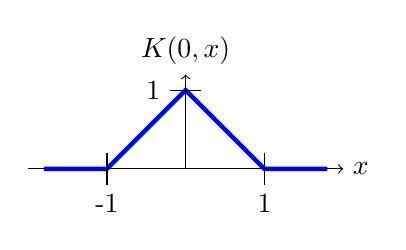
\begin{tikzpicture}[scale=1.0]
  % Axes
  \draw[->] (-2,0) -- (2,0) node[right] {$x$};
  \draw[->] (0,0) -- (0,1.2) node[above] {$K(0,x)$};

  % Kernel function
  \draw[ultra thick, blue] (-1.8,0) -- (-1,0) -- (0,1) -- (1,0) -- (1.8,0);

  % Dashed lines at x = -1 and x = 1
  \draw[-] (-1,0.2) -- (-1,-0.2) node [below] {-1};
  \draw[-] (1,0.2) -- (1,-0.2) node [below] {1};
  \draw[-] (0.2,1) -- (-0.2,1) node [left] {1};
 
\end{tikzpicture}
\caption{Problem \ref{prob:ksmooth1d}.  Triangular kernel}
\label{fig:trik}

\end{figure}


\item \label{prob:knn_cosine} \emph{K-NN with cosine similarity}.  
Consider the following dataset consisting of two-dimensional input vectors and scalar output values:

\begin{center}
\begin{tabular}{|c|c|c|c|c|c|}
\hline
$i$ & 1 & 2 & 3 & 4 & 5 \\ \hline
$x_{i1}$ & 1 & 0 & 1 & 1.5 & 1 \\ \hline
$x_{i2}$ & 0 & 1 & 1 & 1 & 2 \\ \hline
$y_i$ & 2.0 & 2.5 & 3.5 & 5.0 & 4.5 \\ \hline
\end{tabular}
\end{center}

Let the query point be $\bsym{x} = [1.5, 1.5]$. Use cosine similarity to determine the nearest neighbors.
\begin{enumerate}[(a)]
\item Plot the data points $\bsym{x}_i$ in 2D space.  Add the query point $\bsym{x}$ with a different marker.

\item  Compute the cosine similarity between the query point and each data point:
\[
	K(\bsym{x}_i, \bsym{x}) = \frac{\bsym{x}_i^\intercal \bsym{x}}{\|\bsym{x}\|\|\bsym{x}_i\|}
\]

\item Compute the K-NN regression estimate at $\bsym{x}$ by averaging the $y_i$ values of the $K$
 most similar neighbors:
 \begin{itemize} 
 \item $K=1$
 \item $K=2$
 \end{itemize}
\end{enumerate}


\item \emph{Bias and variance}.  Suppose that we have data
\[
	y_i = f_0(x_i) + w_i, \quad w_i \sim \mathcal{N}(0,\sigma^2),
\]
where $f_0(x)$ is the unknown true function:
\[
	f_0(x) = x^2.
\]
Suppose that at some test point $x_0 = 1.3$, we have the estimate 
\[
	\wh{f}(x_0) = \alpha_1 y_1 + \alpha_2 y_2,
\]
with 
\[
	x_1 = 1, \quad x_2 = 2, \quad \alpha_1 = 0.7, \quad \alpha_2 = 0.3.
\]
\begin{enumerate}[(a)]
\item What is the bias: $\mathrm{Bias}(x_0) = f_0(x_0) - \Exp[\wh{f}(x_0)]$
\item What is the variance: $\mathrm{Var}(x_0) = \Exp[ \wh{f}(x_0) - \Exp(\wh{f}(x_0)) ]^2$.
\end{enumerate}



\item \label{prob:ks_pycode} \emph{Kernel smoother implementation}.  
Implement the following function kernel smoother in python. 
Avoid using for-loops for efficient code.
\begin{python}
	def kernel_smoother(Xdat, ydat, X, gam=1.0):
		"""
		Kernel smoother with an RBF kernel
		
		Parameters
		----------
		Xdat:  (ndat,d) array of data inputs
		ydat:  (ndat,) array of data outputs
		X:  (n,d) array of query inputs
		
		Returns
		-------
		yhat: (n,) array of predicted outputs at the queries
		"""
		...
		return yhat
\end{python}


\item \emph{Outlier detection}. Suppose one uses kernel smoothing with an RBF kernel and a query value $\bsym{x}$ satisfies:
\[
	\sum_{i=1}^n K(\bsym{x},\bsym{x}_i) \leq \epsilon,
\]
for some small $\epsilon > 0$.  This condition generally implies that the query sample $\bsym{x}$
is far from all the training data samples $\bsym{x}_i$.  This sort of check can be used to detect
\emph{outliers} that do not follow the training data.  Hence, reliable predictions cannot be made.
Modify the function in Problem~\ref{prob:ks_pycode} to add an output vector \pycode{outlier}
that indicates which samples are outliers.  Use a default value of $\epsilon = 10^{-3}$.


\item \emph{KNN implementation.}  Write a simple function in \pycode{numpy} to implement K-NN.
You can use the function:
\begin{python}
	ind = np.argsort(A, axis=1)  
\end{python} 
which finds the indices for the sorting in each row.  That is,
\begin{python}
	ind[i,k] = index of k-th smallest value in A[i,:]
\end{python}
Use the following function definition:
\begin{python}
	def knn(Xdat, ydat, X,k=1):
		...
		return yhat
\end{python}


\item \label{prob:class1d} 
\emph{Margin in 1d} Consider the data set for four points with
features $\xbf_i=(x_{i1},x_{i2})$ and binary class
labels $y_i=\pm 1$.

\begin{center}
\begin{tabular}{|c|c|c|c|c|c|} \hline
$x_{i1}$ & 0 & 1 & 1 & 2 \\ \hline
$x_{i2}$ & 0 & 0.3 & 0.7 & 1 \\ \hline
$y_i$ & -1 & -1 & 1 & 1 \\ \hline
\end{tabular}
\end{center}

\begin{enumerate}[(a)]
\item Find a linear classifier that separates the two classes.
Your classifier should be of the form
\[
    \hat{y} = \begin{cases}
        1 & \mbox{if } b + w_1 x_1 + w_2 x_2 > 0 \\
        -1 & \mbox{if } b + w_1 x_1 + w_2 x_2 < 0
    \end{cases}
\]
State the intercept $b$ and weights $w_1$ and $w_2$ for your classifier.
Note there is no unique answer as there are multiple linear classifiers
that could separate the classes.


\item Find the maximum $\gamma$ such that
\[
    y_i(b+w_1x_{i1} + w_{i2}x_{i2}) \geq \gamma, \mbox{ for all } i,
\]
for the classifier in part (a)?

\item Compute the margin of the classifier
\[
    m = \frac{\gamma}{\|\wbf\|}, \quad \|\wbf\|= \sqrt{ w_1^2 + w_2^2 }.
\]

\item Which samples $i$ are on the margin for your classifier?
\end{enumerate}



\item \emph{Minimization of the hinge loss}. 
Consider the data set with scalar features $x_i$
and binary class labels $y_i=\pm 1$.

\begin{center}
\begin{tabular}{|c|c|c|c|c|c|c|} \hline
$x_i$ & 0 & 1.3 & 2.1 & 2.8 & 4.2 & 5.7 \\ \hline
$y_i$ & -1 & -1 & -1 & 1 & -1 & 1 \\ \hline
\end{tabular}
\end{center}

Consider a linear classifier for this data of the form,
\[
    \hat{y} = \begin{cases}
        1  & z > 0 \\
        -1 & z < 0,
        \end{cases}
    \quad
    z = x-t,
\]
where $t$ is a threshold.  For each threshold $t$, let $J(t)$
denote the sum hinge loss,
\[
    J(t) = \sum_i \epsilon_i, \quad \epsilon_i = \max(0, 1-y_iz_i).
\]

\begin{enumerate}[(a)]
\item Write a short python program to plot $J(t)$ vs.\ $t$ for
100 values of $t$ in the interval $t \in [0,5]$.

\item Based on the plot, what is one value of $t$ that minimizes
$J(t)$.

\item For the value of $t$ in part (b), find the corresponding
slack variables $\epsilon_i$.

\item Which samples $i$ violate the margin ($\epsilon_i > 0$)
and which samples $i$ are misclassified ($\epsilon_i > 1$).

\end{enumerate}

\item  \emph{Images as matrices}. 
Consider an image recognition problem, where an image $\Xbf$
and filter $\Wbf$ are $4 \x 4$ matrices:
\[
    \Xbf = \left[
        \begin{array}{cccc}
        0 & 0 & 0 & 0 \\
        0 & 0 & 1 & 0 \\
        0 & 0 & 1 & 0 \\
        0 & 0 & 1 & 0
        \end{array} \right], \quad
    \Wbf = \left[
        \begin{array}{cccc}
        0 & 0 & 0 & 0 \\
        0 & 1 & 1 & 0 \\
        0 & 1 & 1 & 0 \\
        0 & 0 & 0 & 0
        \end{array} \right].
\]
\begin{enumerate}[(a)]
\item Recall that in linear classification, the $4 \x 4$
image matrices $\Xbf$ and $\Wbf$
can be represented as 16-dimensional vectors, $\xbf = \mathrm{vec}(\Xbf)$
and $\wbf = \mathrm{vec}(\Wbf)$ by stacking the columns of the matrices
vertically. What are $\xbf$ and $\wbf$ for the matrices above.

\item What is the inner product $z = \wbf\tran \xbf$.

\item What is the inner product $z = \wbf\tran \xbf_{\rm right}$ where
$\xbf_{\rm right}$ is
the vector corresponding to the matrix $\Xbf$ right shifted by one pixel
with the left column filled with zeros.

\item What is the inner product $z = \wbf\tran \xbf_{\rm left}$ where
$\xbf_{\rm left}$ is
the vector corresponding to the matrix $\Xbf$ left shifted by one pixel
with the right column filled with zeros.

\item Write the python command that can covert a $4 \x 4$ image matrix, \pycode{Xmat}
to the 16-dimensional vector, \pycode{x}.  What is the python command
to go from \pycode{x} to \pycode{Xmat}.
\end{enumerate}







\item \label{prob:rbf}
Consider the data set with scalar features $x_i$
and binary class labels $y_i=\pm 1$.

\begin{center}
\begin{tabular}{|c|c|c|c|c|} \hline
$x_i$ & 0 & 1 & 2 & 3 \\ \hline
$y_i$ & 1 & -1 & 1 & -1 \\ \hline
\end{tabular}
\end{center}

A support vector classifier is of the form
\[
    \hat{y} = \begin{cases}
        1  & z > 0 \\
        -1 & z < 0,
        \end{cases}
    \quad
    z = \sum_i \alpha_i y_i K(x_i,x),
\]
where $K(x,x')$ is the radial basis function, $K(x,x') = e^{-\gamma(x-x')^2}$, and
$\gamma > 0$ and $\alphabf = [\alpha_1,\ldots,\alpha_4]$ are parameters of the classifier.

\begin{enumerate}[(a)]
\item Use python to plot $z$ vs.\ $x$ and
$\hat{y}$ vs.\ $x$ when $\gamma = 3$ and $\alphabf = [0,0,1,1]$.
\item Repeat (a) with $\gamma = 0.3$ and $\alphabf = [1,1,1,1]$.
\item Which classifier makes more errors on the training data.
\end{enumerate}

\end{enumerate}


\end{document}

